\documentclass[10pt,a4paper]{article}
\usepackage[utf8]{inputenc}
\usepackage{amsmath}
\usepackage{amsfonts}
\usepackage{amssymb}
\usepackage{a4wide} %Wider margins
\usepackage[english]{babel} %English dictionary for hyphenation and definitions, e.g. Table vs. Tabel
\usepackage[official]{eurosym} %Support for Euro-sign
\usepackage[utf8]{inputenc} %Support for internationalization, e.g. é vs.\’e
\usepackage{amsmath,amssymb,amsthm} %Support for mathematical formulas and symbols
\usepackage{fancyhdr} %Fancy headers
\usepackage{hyperref} %Creates clickable links
\usepackage{graphicx} %Support for grahpics
\usepackage{nopageno} %Support for removal of pagenumbers
\usepackage{tabularx}
\usepackage{enumitem}
\usepackage{xspace}
\usepackage{algorithm,algpseudocode}
\usepackage{float}
\usepackage{mathtools}
\usepackage[dvipsnames]{xcolor}
\usepackage[titletoc,toc,title]{appendix}
\usepackage{listings}
\usepackage{pdfpages}
\usepackage{footmisc}
\usepackage{attachfile2}
\usepackage{subfig}
\graphicspath{ {./ThesisFigures/} }

\hypersetup{
    pdftitle={}, %PDF-file will be given a proper title when viewed in a reader
    hidelinks %PDF-file will be given clickable, yet not visible links when viewed in a reader
}
\newcommand{\documenttitle}{Skin Disease Basic Analysis}
\newcommand{\documentsubtitle}{A case study for a computational biology framework}


\newcommand{\true}{{\sc True}\xspace}
\begin{document}
	
	\begin{titlepage}
		
		\center
		
		\vspace*{3cm}
		
		\textbf{\huge \documenttitle}
		
		\textit{\LARGE \documentsubtitle}
		
		\vspace*{2cm}
		
		\large
		\centering
		T.P.A.~\textsc{Beishuizen}~(0791613)\\
		Biomedical Engineering - Computational Biology\\
		Computer Science - Data Mining\\
		Eindhoven, University of Technology\\
		Email: \texttt{t.p.a.beishuizen@student.tue.nl}
		
		\vfill
		
		\vspace*{1cm}
		
		\today
		
	\end{titlepage}
	
	\tableofcontents
	
	%\newpage
	
	\pagestyle{fancy}
	%Abbreviations used by fancyhdr:
	%E Even page
	%O Odd page
	%L Left field
	%C Center field
	%R Right field
	%H Header
	%F Footer
	\fancyhead{} % clear all header fields
	\fancyfoot{} % clear all footer fields
	\renewcommand{\headrulewidth}{0.4pt}
	\renewcommand{\footrulewidth}{0.4pt}
	
	\fancyhead[L]{\rightmark}
	\fancyfoot[C]{\thepage}
	\fancyhead[R]{T.P.A. Beishuizen}
	
	
	\clearpage
	
	\section{Introduction}
	\label{sec:Introduction}
	
	% Quick explanation for biomedical data
	Biomedical Engineers are known to extract useful information out of biomedical data. The biomedical data can come from many different sources: hospitals, universities and private companies, but also publicly available data. Currently, a standard is missing to analyse those datasets efficiently. 

	% Explanation skin disease data
	An example of biomedical data is a set based on gene expression of skin diseases\cite{nair2009genome, suarez2012expanding, bigler2013cross, kim2016spectrum, yao2008type, suarez2011nonlesional, tintle2011reversal, gittler2012progressive}. Two skin diseases were tested, psoriasis and atopic dermatitis. The expression numerous of genes was tested for skin disease patients on skin affected by the disease (lesional skin) and skin not affected by the disease (non-lesional skin). Further data from healthy subjects was also acquired. Nine datasets were available, six for psoriasis\cite{nair2009genome, suarez2012expanding, bigler2013cross, kim2016spectrum, yao2008type} and three for atopic dermatitis\cite{suarez2011nonlesional, tintle2011reversal, gittler2012progressive}. The number of tested skin biopies ranged from 28 to 180 whereas the number of tested genes is the same for every set, namely 54675.

	% Explanation skin data analysis
	With the vast number of datasets that are available, such a standard in the form of a framework on data analysis would be valuable. This framework can be a basis for researchers to start with their data analysis preventing them from creating everything from scratch. In this project, a basic analysis was done on the available skin disease datasets, as a case study for creating a framework for biomedical engineers. First, a background is given on the dataset. Secondly, methods to extract information from the data were explained, followed by their results. At last, conclusions are made using the found results and useful aspects for a biomedical engineering framework about the basic analysis are discussed.
	
	
	\section{Skin Diseases Datasets}
	\label{sec:SkinDiseasesDataSet}
	
	% Introduction
	Skin diseases can have a major impact in someone's life. Whereas skin diseases are not as life threatening as diseases such as cancer, Alzheimer and AIDS, they can lower quality of life significantly. When looking at the health-related quality of life (HRQL), patients with psoriasis show the same problems as patients with other major chronic health conditions\cite{rapp1999psoriasis}. Patients with both psoriasis and atopic dermatitis suffer from severe itching and pains. Further insights into the skin diseases can help alleviate their unwanted side-effects and help improve the patients' quality of life\cite{jowett1985skin}.
	
	% Dataset introduction
	Information on both of these skin diseases can be found in nine datasets stored on the NCBI database\cite{edgar2002gene}. The datasets comprise microarray data extracted biopsies of psoriasis patients, both from their lesional and non-lesional skin. In several experiments this skin is taken from the same patient. Also some skin is taken from patients not suffering from the diseases at all. six datasets focus on Psoriasis and three focus on atopic dermatitis. These datasets consist of a total number of 54675 genes, the features of the dataset. The range of acquired samples varies among datasets from 28 tot 180. Also, since every dataset was created by different people, some minor differences can be present in them as well (Table \ref{tab:SkinDiseasesDataSets}), due to different measurement equipment.
	
	\begin{table}[h!]
		\centering
		\caption{Details of the nine skin disease datasets. The number of samples and genes has been given, as well as remarks of the skin types.}
		\label{tab:SkinDiseasesDataSets}
		\begin{tabular}{cc|ccl}
			\textbf{Disease}                                                     & \textbf{Dataset name} & \textbf{Sample size} & \textbf{Genes} & \textbf{Remarks}                                                                                                                                                                                                                                        \\ \hline
			\textbf{Psoriasis}                                                   & \textbf{GSE13355} \cite{nair2009genome}      & 180                  & 54675             & \begin{tabular}[c]{@{}l@{}}Three skin types: \\ - NN (normal, 64 samples)\\ - PN  (non-lesional, 58 samples) \\ - PP (lesional, 58 samples)\end{tabular} \\ \cline{3-5} 
			\textbf{}                                                            & \textbf{GSE30999} \cite{suarez2012expanding}      & 170                  & 54675             & \begin{tabular}[c]{@{}l@{}}- No normal patients\\ - Non-lesional (85 samples)\\ - Lesional (85 samples)\end{tabular}                                                                                                                    \\ \cline{3-5} 
			\textbf{}                                                            & \textbf{GSE34248} \cite{bigler2013cross}      & 28                   & 54675             & \begin{tabular}[c]{@{}l@{}}- No normal patients\\ - Non-lesional (14 samples)\\ - Lesional (14 samples)\end{tabular}                                                                                                                              \\ \cline{3-5} 
			\textbf{}                                                            & \textbf{GSE41662} \cite{bigler2013cross}      & 48                   & 54675             & \begin{tabular}[c]{@{}l@{}}- No normal patients\\ - Non-lesional (24 samples)\\ - Lesional (24 samples)\end{tabular}                                                                                                                               \\ \cline{3-5} 
			\textbf{}                                                            & \textbf{GSE78097} \cite{kim2016spectrum}      & 33                   & 54675             & \begin{tabular}[c]{@{}l@{}}Different types of skin samples: \\ - Normal (6 samples)\\ - Mild Psoriasis (14 samples) \\ - Severe Psoriasis (13 samples)\end{tabular}                                                                                \\ \cline{3-5} 
			\textbf{}                                                            & \textbf{GSE14905} \cite{yao2008type}     & 82                   & 54675             & \begin{tabular}[c]{@{}l@{}}- Normal skin (21 samples), \\ - Non-lesional skin (28 samples)\\ - Lesional skin (33 samples)\end{tabular}                                                                                                                 \\ \hline
			\textbf{\begin{tabular}[c]{@{}c@{}}Atopic\\ Dermatitis\end{tabular}} & \textbf{GSE32924} \cite{suarez2011nonlesional}      & 33                   & 54675             & \begin{tabular}[c]{@{}l@{}}- Normal skin (8 samples) \\ - Non-lesional skin (12 samples)\\ - Lesional skin (13 samples)\end{tabular}                                                                                                         \\ \cline{3-5} 
			\textbf{}                                                            & \textbf{GSE27887} \cite{tintle2011reversal}      & 35                   & 54675             & \begin{tabular}[c]{@{}l@{}}Different type of skin samples, \\ pre and post treatment of skin: \\ - Pre non-lesional (8 samples)\\ - Post non-lesional (9 samples)\\ - Pre lesional (9 samples)\\ - Post lesional (9 samples)\end{tabular}       \\ \cline{3-5} 
			\textbf{}                                                            & \textbf{GSE36842} \cite{gittler2012progressive}      & 39                   & 54675             & \begin{tabular}[c]{@{}l@{}}Also difference between \\ acute and chronic dermatitis. \\ - Normal (15 samples)\\ - Non-lesional (8 samples) \\ - Acute lesional (8 samples) \\ - Chronic lesional (8 samples)\end{tabular}                    \\ \cline{1-5} 
		\end{tabular}
	\end{table}
	
	% Introduction challenges
	The nine datasets are rich in information. The dimensionality is very high and if combined the datasets also have a decent number of samples. Several challenges arise in the dataset, too, as in biomedical datasets often have. Here, three of these challenges are discussed.
	
	% Challenge 1: Data heterogeneity
	At first the challenge of handling nine different datasets is essential. Even though the genes were chosen according to the Affymetrix Human Genome\cite{dixon2007genome}, the layouts are not identical. These difference originate from the intended research goals and the data availability. It is not possible to just concatenate samples without some form of preprocessing. Only the parts that are the same all over the datasets must be taken and all other parts omitted.
	
	% Challenge 2: Data dimensionality
	A second challenge can be found in the high number of genes. There were 74675 genes measured, averaged at about 1000 times the number of samples. The genes that are significantly involved in the skin diseases however is estimated to be about $1/1000^{th}$ of the total number of measured genes. Many genes are redundant and can be removed during preprocessing, a valuable and complex step in biomedical data mining.
	
	% Challenge 4: Data Volume
	The third challenge is about data volume. The number of samples differs from 28 to 180, all of them being a very low number compared with the number of genes. This indicates that the number of samples represent the complete sample space poorly and will not show the thresholds between lesional and non-lesional skin clearly. This can create problems, mainly during machine learning, with such a low training and test set. Several cases will arise where all training and test set agree with the algorithm, whereas other samples from the sample space would not.
	
	\subsection{Additional Data}
	\label{subsec:AdditionalData}
	
	% To write: Something about the additional data
	The genes all correspond to the same genes for all of these nine different datasets. The NCBI database\cite{edgar2002gene} also provides separate data containing substantial information for every gene. This information includes gene ID, commonly known name and abbreviation and which gene database it originates from. It also contains processes and molecular reactions the gene is involved with, as well as the location of it in the cell.. This data can be used to find links between several processes and their corresponding genes.
	
	\section{Methods}
	\label{sec:Methods}
	
	% Methods introduction
	Three different aspects are investigated with the dataset. At first several techniques are used to reduce the high number of genes. Secondly the genes (either before feature reduction or after) are clustered. Thirdly all genes of psoriasis and atopic dermatitis are compared after reducing them, to find whether genes were over expressed in both of them.
	
	% Non-Lesional vs Lesional
	A previous project\footnote{BEP Project -\textit{ Manouk Groels}} found out that healthy and non-lesional skin do not show many differences and after some testing, the same conclusion is reached in teh current study. Aside from this, the difference between lesional and non-lesional skin is the most important for skin diseases to compute, as that difference shows which genes are over- or underexpressed in lesional skin. Therefore the main focus of the project was showing the difference between non-lesional and lesional skin in terms of genes. 
	
	% Only best Psoriasis sets
	For the computation of feature reduction, the largest possible dataset was created with only non-lesional and lesional skin samples. The biggest dataset that could be created was with the Psoriasis sets that had both non-lesional and lesional skin (table \ref{tab:SkinDiseasesDataSets}), good for a total of 423 samples. When comparing Psoriasis and Atopic Dermatitis, all suitable samples of Atopic Dermatitis were collected for a total of 58 samples. In gene reduction and clustering only the Psoriasis dataset is used, due to its bigger size. When comparing Psoriasis and Atopic Dermatitis, both are used.
	
	\subsection{Feature Reduction}
	\label{subsec:MethodsFeatureReduction}
	
	% Introduction
	Since the number of features in the data is 54675 (the number of genes), a significant feature reduction is needed before any meaningful computations could be done. Therefore two different ways of feature reduction were explored. The first one was doing a simple t-test to find all genes that were significantly different. The second one was testing correlation between all genes, also known as multicollinearity testing.
	
	% T-test SciPy
	For using a t-test, the SciPy package ise used. For the t-test three different possibilities were available, one for paired data, one for data with equal variance and one for data with unequal variance.\footnote{\label{fn:BDA}Biomedical Data Analysis - \textit{Tim Beishuizen}} In this case, all but one dataset (GSE14905) were paired and no variances were known so unpaired data with unequal variance was used.
	
	% Multicollinearity
	To test whether genes are correlated, multicollinearity should be tested. Usually this would be computed by calculating the correlation coefficient between all genes. This coefficient was quite heavy computationally to compute and therefore took up too many memory space for a cpu. A greedy hands on approach to remove multicollinearity is done by testing all genes for their correlation coefficient and removing the least significant one if they correlate high enough.
	
	% Machine Learning RandomForest
	After removing the unuseable genes and multicollinearity, a random forest classifier from the scikit-learn package is used to find out whether removing unuseable genes and multicollinearity actually improves the possibility to better classify lesional skin. Both the gene sets before and after removal are tested with a decision tree classifier. For this classification a cross validation is done with 100 different subsets. After testing with a decision tree classifier a random forest classifier was also used. From the random forest classifier, all genes that were used multiple times as a splitting criterium were extracted to find out if the classifier used genes multiple times.
	
	\subsection{Clustering}
	\label{subsec:MethodsPositionalClustering}
	
	% Introduction
	With the high number of genes even after feature reduction, cluster is a good way to find whether genes show similar behaviour. This clustering can be done in two different ways. The first way is based the values of the genes, clustering genes that show the same behaviour. A second way is clustering them by checking biomedical relations between the genes. Both possibilities were worked used to find interesting results.
	
	% Standardization
	Before clustering was done though, the values were standardized per sample. This standardization is done to remove high differences in especially variation. Two types of standardization are done: by gene and by sample. At first standardization per genes is done, so every gene is treated equally. Relative big differences in gene expression are shown that way. Standardization of variance per sample gives skin cell specific genes higher values than non-skin cell specific genes, because their expression should be higher overall. This way genes known to be more prevalent in skin cells have a higher chance to be noticed for the difference between lesional and non-lesional skin.
	
	% Clustering types
	The first type of clustering is done by using basic clustering methods. Three different types of clustering were used: K-means, Agglomerative and DBSCAN, all three of them methods in scikit-learn. K-means tries to cluster the genes in $k$ groups of equal variance. Agglomerative clustering is also known as hierarchical bottom-up clustering, in which clusters are merged until the desired number of clusters is left. DBSCAN tries to divide the genes in clusters with high density and works best with a high number of values combined with a low number of clusters. For both K-means and agglomerative clustering a variation of cluster numbers are chosen to find the best possible selection. 
	
	% Process/Cellular/Molecular
	Aside from clustering the genes by values, another way is clustering by biomedical relations. The additional dataset (subsection \ref{subsec:AdditionalData}) links genes to three different biomedical components: processes, cellular locations and molecular reactions. Genes linked to the same process means the genes are involved in that particular process and therefore can be clustered together. An example of such a process is keratinization. Cellular locations show which location the product of gene translation is active in, for example in the cytoplasma. Genes linked to molecular reactions means they are linked to the same reaction in the body, for example enzym binding. Since genes can be linked to multiple processes, locations and reactions, they can be put in multiple clusters for all three.
	
	% Combining clusters
	Both types of clustering should give different results, as one of them only takes into account the values and while the other focuses on biomedical relations. A good way to find results is to combine both clustering types, to find out which value clusters also are involved in similar biomedical processes. This is done by first selecting value dependent clusters and then searching for matching biomedical relations within the clusters.
	
	\subsection{Psoriasis Versus Atopic Dermatitis}
	\label{subsec:MethodsPsoriasisVersusAtopicDermatitis}
	
	% Also took AD sets
	At last a brief search for the difference between Psoriasis and Atopic Dermatitis is done. Since up- and down regulations for both of these diseases are more interested, first feature reduction is done by only choosing the ones that showed a significant difference. The genes for both diseases are then compared and for all genes that are up- or down regulated for both diseases, all biomedical processes, cellular locations and molecular reactions are extracted and counted how many times they were present for both diseases. 
	
	\section{Results}
	\label{sec:Results}
	
	% Results introduction
	The results are split in the same way as the methods was split. First the results for feature reduction are shown for t-test, multicollinearity as well as for the machine learning improvements. Secondly the results for clustering are shown. Emphasis was put for combining clustering by value and clustering by biomedical relations. At last the similarities between Psoriasis and Atopic Dermatitis were shown to see if genes, processes, cellular locations and molecular reactions are involved in both diseases. 
	
	
	\subsection{Feature Reduction}
	\label{subsec:ResultsFeatureResuction}
	
	% T-test SciPy
	The t-test is used between non-lesional and lesional skin for every dataset separately and combined (Table \ref{tab:FeatureReduction}). A low p-value of $p=0.001$ is chosen by trial and error. Interestingly enough when all datasets are combined, the number of significant features is lower than when looking at the datasets separately. This can indicate that dataset specific noise is present in the datasets and heterogeneity actually improves noise reduction. After this feature reduction, further computation is done with the 1768 genes left.
	
	\begin{table}[H]
		\centering
		\caption{The results of using the t-test for genes in all relevant Psoriasis datasets separately and combined. A paired t-test is done if applicable, otherwise an unknown variance unpaired t-test is done. The number of samples for both lesional and non-lesional skin is shown additionally.}
		\label{tab:FeatureReduction}
		\begin{tabular}{l|ccc|cc}
			\textbf{Dataset} & \textbf{\begin{tabular}[c]{@{}c@{}}Samples \\ Lesional Skin\end{tabular}}                                  & \textbf{\begin{tabular}[c]{@{}c@{}}Samples\\ Non-Lesional Skin\end{tabular}}  & \textbf{Paired} & \textbf{All Genes} & \textbf{\begin{tabular}[c]{@{}c@{}}Significant\\ Genes\end{tabular}} \\ \hline
			GSE13355          & 58                                            & 58                                                & Yes    & 54675              & 22106                      \\
			GSE30999          & 85                                            & 85                                                & Yes    & 54675              & 20836                      \\
			GSE34248          & 14                                            & 14                                                & Yes    & 54675              & 7824                       \\
			GSE41662          & 24                                            & 24                                                & Yes    & 54675              & 15672                      \\
			GSE14905          & 33                                            & 28                                                & No     & 54675              & 13355                      \\ \hline
			Combined          & 214                                           & 209                                               & No     & 54675              & 1768                      
		\end{tabular}
	\end{table}
	
	
	% Multicollinearity
	Computing multicollinearity after some testing and literature research a value of $0.7$ is chosen as a threshold whether two values showed enough correlation. Greedy clustering creates 335 clusters for the combined dataset, so for 335 genes the correlation coefficient is lower than $0.7$ between all of them. The ability to find the difference between lesional and non lesional skin with a Decision tree classifier shows that only using significant genes gives the best results, whereas using the uncorrelated genes makes both the validation as the test score worse. (Table \ref{tab:DecisionTreeResults}).
	
	\begin{table}[H]
		\centering
		\caption{The results of the decision tree classifier for different sets of genes: all genes, only the significant genes and the uncorrelated genes. The decision tree was cross validated by division in 100 different subsets and afterwards tested by a separate test set.}
		\label{tab:DecisionTreeResults}
		\begin{tabular}{l|ccc}
			\textbf{Gene set}                                            & \textbf{Genes} & \textbf{Validation score} & \textbf{Test score} \\ \hline
			All genes                                                    & 54675             & 0.584                     & 0.575               \\
			Significant genes                                            & 1768              & 0.959                     & 0.943               \\
			Uncorrelated genes & 335               & 0.928                     & 0.915              
		\end{tabular}
	\end{table}
	
	% RandomForest
	With a validation and test score of around 0.95, the significant gene set is used for a random forest classification consisting of a 1000 decision trees. The genes that were used as splitting criteria for these decision trees are collected to find out whether the same genes pop up multiple times as the best splitting criteria (Table \ref{tab:GeneRandomForestOccurence}). While the number of multiple occurrences is not as high as expected, the six most occurring genes already show to have some kind of relation with skin diseases. 
	

\begin{table}[H]
	\centering
	\caption{The six most used genes as splitting criteria for the random forest classifier. The genes are also compared with literature.}
	\label{tab:GeneRandomForestOccurence}
	\begin{tabular}{l|ccc}
		\textbf{Gene ID} & \textbf{Gene Title}                                                                                        & \multicolumn{1}{l}{\textbf{\begin{tabular}[c]{@{}l@{}}Times used in\\ random forest\end{tabular}}} & \textbf{Link with Psoriasis}                                                                                         \\ \hline
		NM\_004262       & \begin{tabular}[c]{@{}c@{}}transmembrane protease, \\ serine 11D\end{tabular}                              & 45                                                                                                 & \begin{tabular}[c]{@{}c@{}}Previously discovered \\ relation with Psoriasis\cite{suarez2012expanding}\end{tabular} \\ \hline
		AI186548         & keratin 77                                                                                                 & 33                                                                                                 & \begin{tabular}[c]{@{}c@{}}Keratin is upregulated in \\ uncontrollable growth skin cells\cite{suarez2012expanding}\end{tabular}           \\     \hline
		BF032500         & MACRO domain containing 2                                                                                  & 33                                                                                                 & \begin{tabular}[c]{@{}c@{}}Previously discovered \\ relation with Psoriasis\cite{suarez2012expanding}\end{tabular}                             \\ \hline
		NM\_001062       & \begin{tabular}[c]{@{}c@{}}transcobalamin I (vitamin B12 \\ binding protein, R binder family)\end{tabular} & 31                                                                                                 & \begin{tabular}[c]{@{}c@{}}Previously discovered \\ relation with Psoriasis\cite{suarez2012expanding}\end{tabular} \\ \hline
		NM\_005621       & S100 calcium binding protein A12                                                                           & 31                                                                                                 & \begin{tabular}[c]{@{}c@{}}Previously discovered \\ relation with Psoriasis\cite{suarez2012expanding}\end{tabular} \\ \hline
		U19557           & \begin{tabular}[c]{@{}c@{}}serpin peptidase inhibitor, \\ clade B (ovalbumin), member 3 \& 4\end{tabular}  & 31                                                                                                 & \begin{tabular}[c]{@{}c@{}}Previously discovered \\ relation with Psoriasis\cite{suarez2012expanding}\end{tabular}
	\end{tabular}
\end{table}
	
	\subsection{Clustering}
	\label{subsec:ResultsPositionalClustering}
	
	% Process/Cellular/Molecular clustering
	Only the 1768 significant genes found from feature reduction are used for clustering. The genes are clustered per process, cellular location and molecular reaction they are linked to, so if two genes are both related to a certain process, they are clustered together. Since a gene can be linked to multiple processes, it can also be present in multiple clusters. The processes, cellular locations and molecular reactions are ordered by averaging the difference in gene expression for the genes in their cluster, meaning a higher averaging difference corresponds to a higher score. The sixteen highest scoring processes (appendix \ref{app:BiomedicalClusters} and figure \ref{fig:ProcessesScaledBySample}), cellular locations (appendix \ref{app:BiomedicalClusters}) and molecular reactions (appendix \ref{app:BiomedicalClusters}) are shown for scaling per gene and scaling per sample. After showing these results to an expert\footnote{\label{fn:Felix}MsC. Felix Garza - University of Technology Eindhoven}, the cellular locations and molecular reaction did not show any interesting results. The interesting results were found in several interesting processes, related to inflamatory response:
	
	\begin{enumerate}
		\item[-] acute inflammatory response
		\item[-] regulation of inflammatory response 
		\item[-] response to interferon gamma 
		\item[-] chronic inflammatory response
		\item[-] oxidative stress.
	\end{enumerate}
	
	% Insert figures
	\begin{figure}[H]
	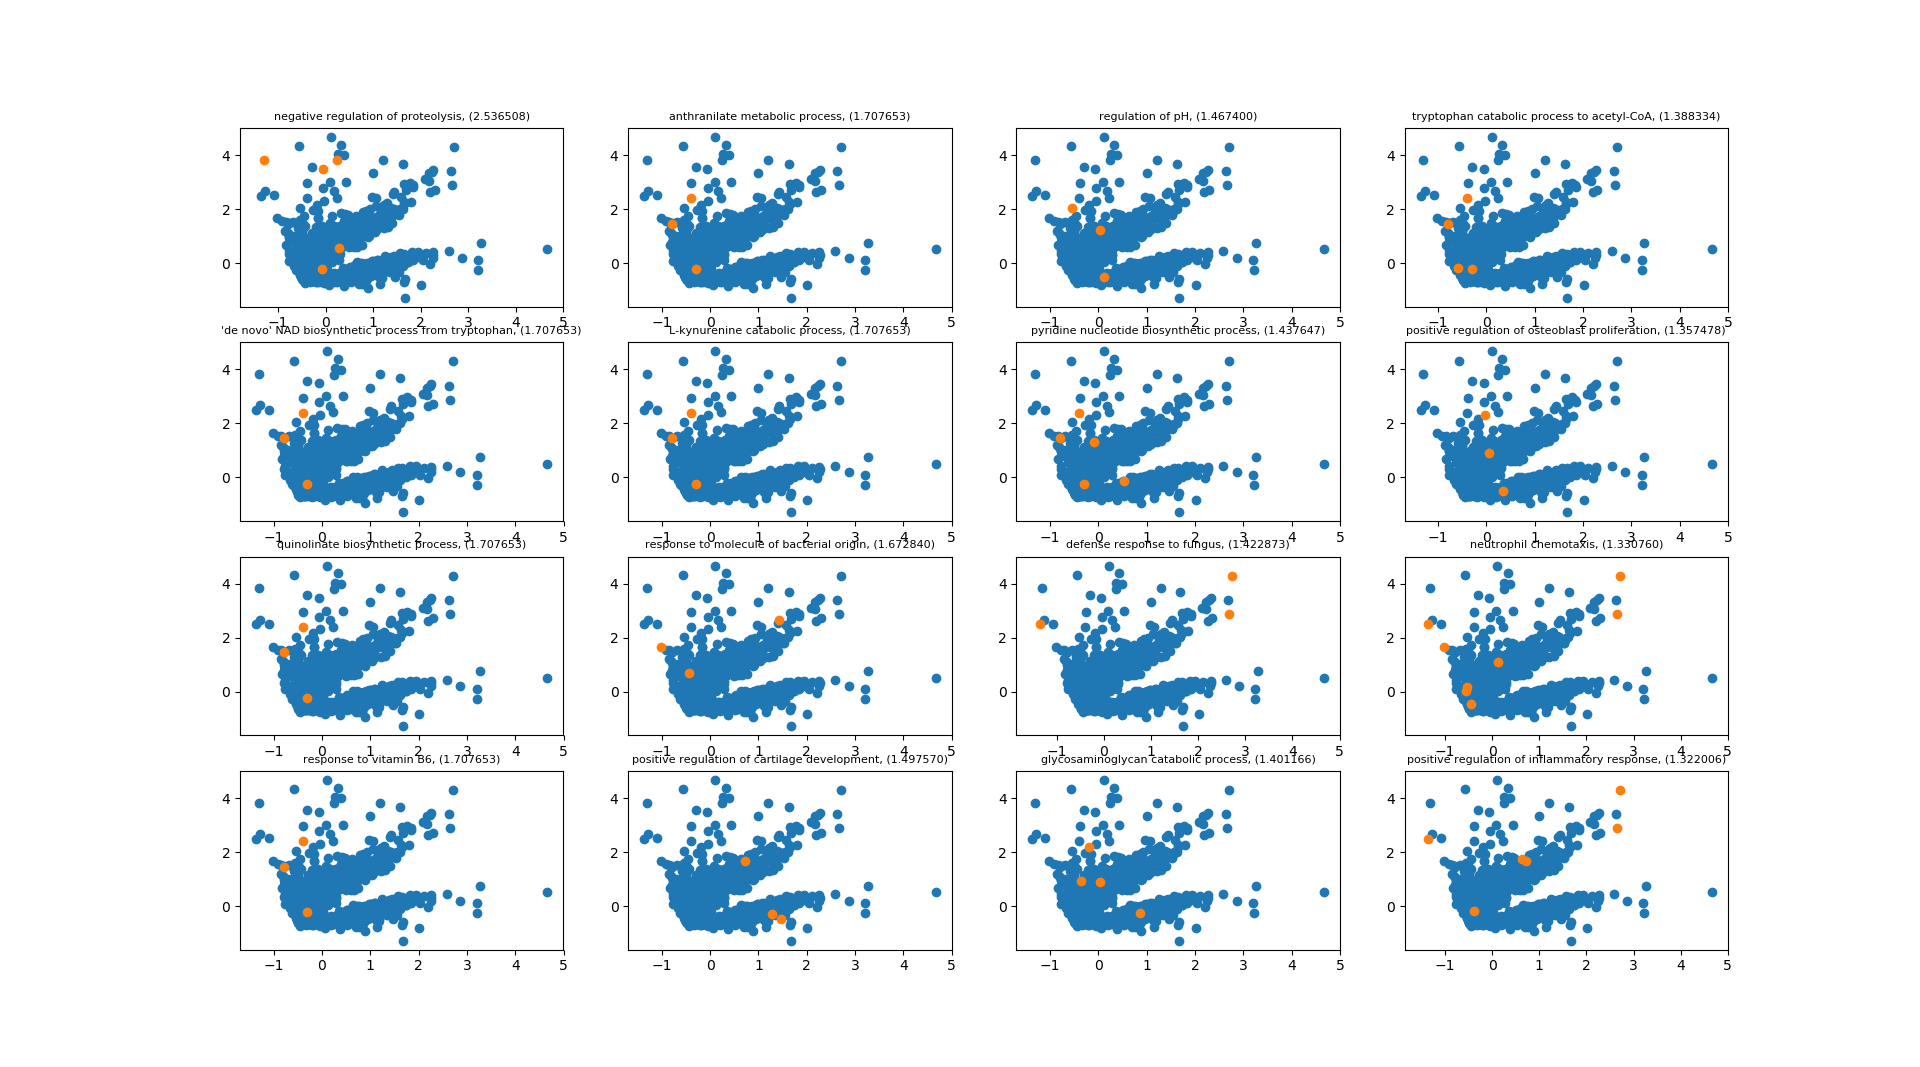
\includegraphics[width=1\textwidth]{Sign_Processes_Psoriasis.png}
	\label{fig:ProcessesScaledBySample}
	\caption{The 16 processes that show the highest difference in gene expression between lesional and non-lesional data. The data is standardized by sample and orange points are genes that are related to the process, Blue dots are genes unrelated to the process}
\end{figure}	
	
	% Clustering types
	Cross-referencing the value-based clustering and the biomedical relation clustering, agglomerative clustering with ten clusters gives the best results.(Figure \ref{fig:ClusteredGenes}). After linking the genes with biochemical processes, cluster 5 and cluster 8 show interesting links in results. Cluster 5 is linked to multiple processes typically occurring in skin cells, for example involving keratin and the epidermis. Cluster 8 is linked to multiple processes involving negative regulation of several enzymes, for example endopeptidase, peptidase and proteolysis. Other clusters are linked to less specific processes, for example to transport and protein binding.
	
	\begin{figure}[H]
		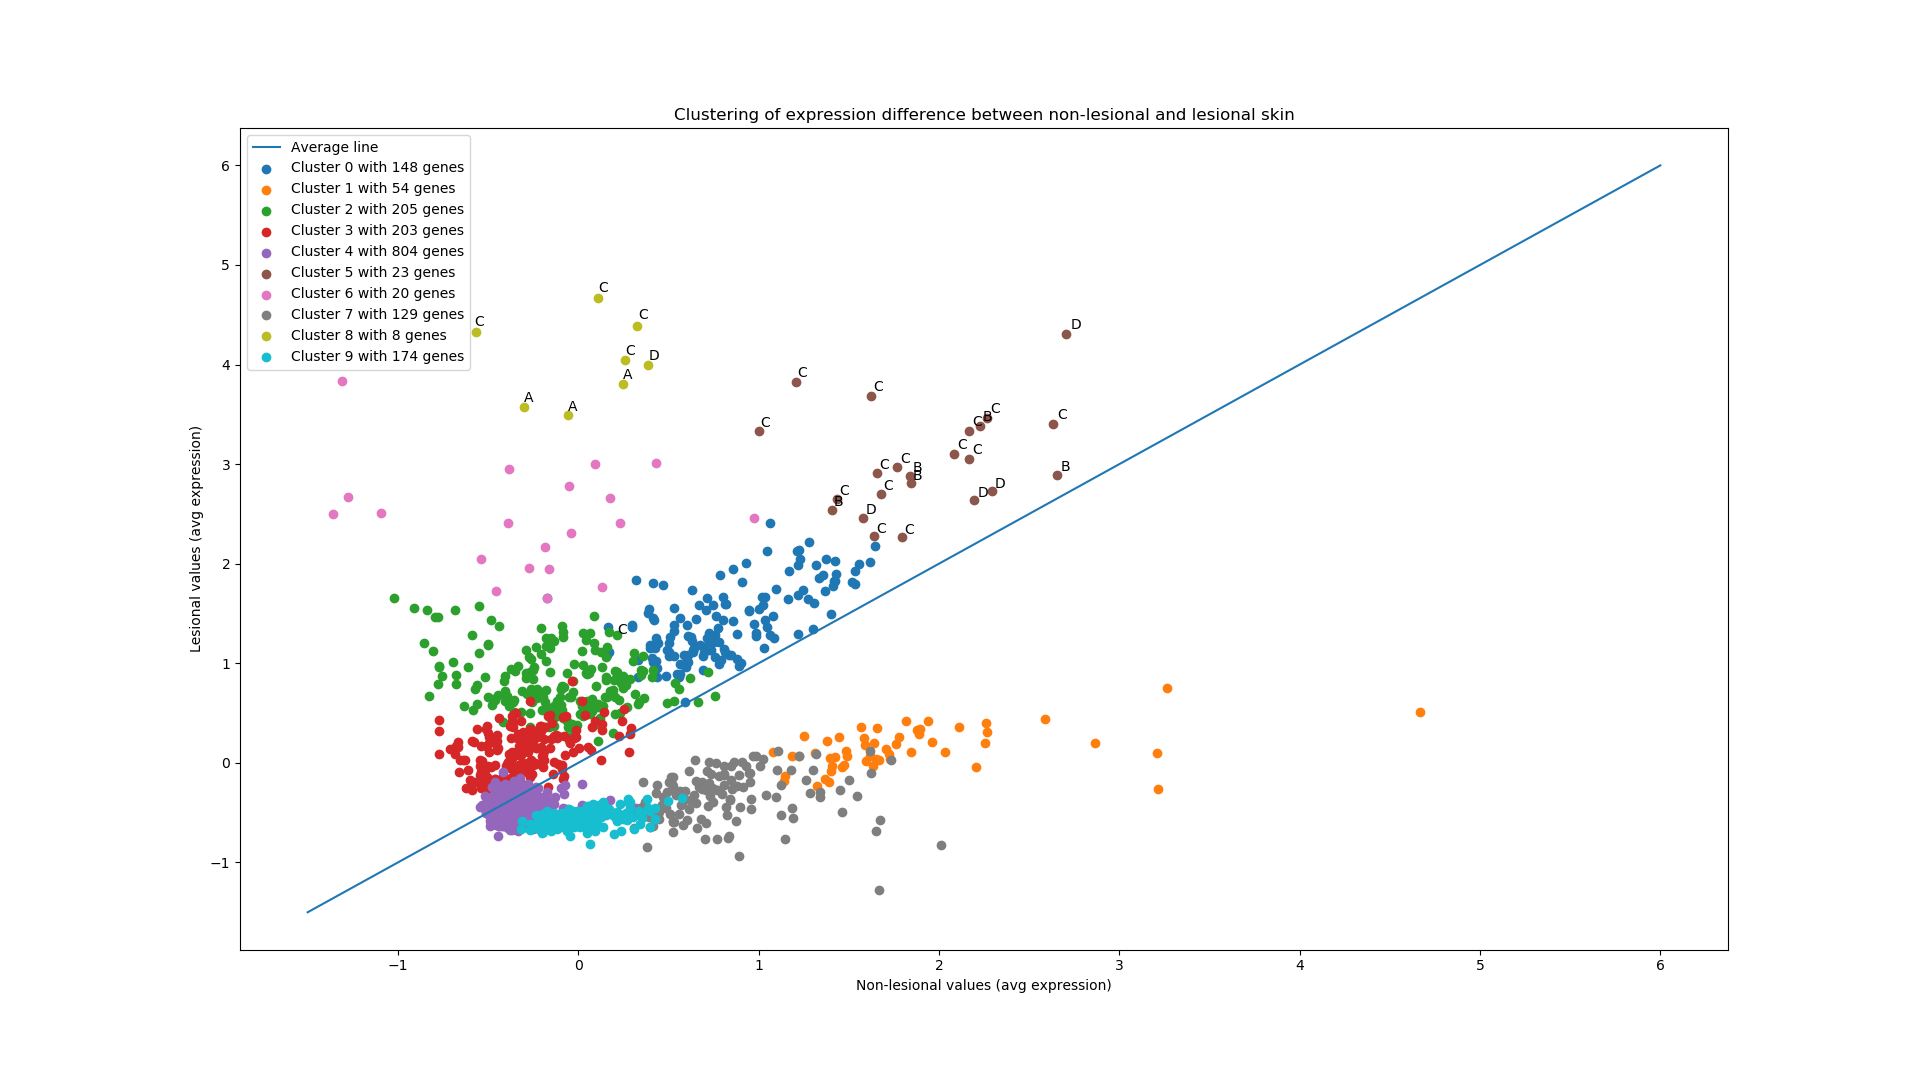
\includegraphics[width=\textwidth]{10_Clusters_Psoriasis_Results.png}
	
		\caption{10 different clusters found by agglomerative clustering for the Psoriasis dataset. The data points are genes that showed a significant difference in expression between lesional (y-axis) and non-lesional (x-axis) skin and standardized per sample. Cluster 5 and 8 show the most useful genes and are also marked for Psoriasis relevance: Known Psoriasis marker (A), Known to be upregulated for Psoriasis (B), Known to be upregulated for uncontrollable growth (C) and unknown relation (D)}
		\label{fig:ClusteredGenes}
	\end{figure}
	
	% Specific look at interesting clusters
	Since cluster 5 and 8 give interesting results on a process level, an expert on psoriasis gene expression\footref{fn:Felix} was asked to label all genes in clusters 5 and 8. Most of the genes in these clusters can be linked to Psoriasis directly or indirectly (Figure \ref{fig:ClusteredGenes}).
	
	\subsection{Psoriasis Versus Atopic Dermatitis}
	\label{subsec:ResultsPsoriasisVersusAtopicDermatitis}
	
	% Also took AD sets
	At last the significant genes for Atopic Dermatitis are compared with the significant genes of Psoriasis (Table \ref{tab:ConditionsPsoriasisAD}). After matching both datasets to find out whether any genes are significant in both datasets, 96 genes are left. These genes are linked to processes to find processes that show differences between lesional and non-lesional skin in both Psoriasis and Atopic Dermatitis. Five processes give the biggest result, however, all of these processes seem basic and therefore not useful for further investigation:
	
	\begin{enumerate}
		\item[-] metabolic process
		\item[-] small molecule metabolic process
		\item[-] regulation of transcription, DNA-templated
		\item[-] signal transduction
		\item[-] transcription, DNA-templated
	\end{enumerate}
	
	\begin{table}[H]
		\centering
		\caption{The initial conditions of the Psoriasis and Atopic Dermatitis datasets}
		\label{tab:ConditionsPsoriasisAD}
		\begin{tabular}{r|cccc}
			\textbf{Dataset} & \textbf{\begin{tabular}[c]{@{}c@{}}Samples\\ Lesional Skin\end{tabular}} & \textbf{\begin{tabular}[c]{@{}c@{}}Samples\\ Non-Lesional Skin\end{tabular}} & \textbf{All Genes} & \textbf{Significant Genes} \\ \hline
			Psoriasis         & 214                                                                      & 209                                                                          & 54675                 & 1768                          \\
			Atopic Dermatitis & 30                                                                       & 28                                                                           & 54675                 & 516                          
		\end{tabular}
	\end{table}
	
	\section{Discussion}
	\label{sec:Conclusion}
	
	% Introduction conclusion
	Three different aspects have been researched: feature reduction, clustering and comparing Psoriasis and Atopic Dermatitis. Some results do not give any additional insights, however others actually show possible future research topics.
	
	% Feature reduction
	Using a t-test seemed to be an effective way to reduce the number of genes significantly without any loss in information. Especially for multiple and bigger datasets this method was effective for Psoriasis. The loss in information was present however when using the greedy correlation method, which was not used in further computations because of that information loss. After computing which genes would be used as splitting criteria, the six most occuring genes all but one either can be found in literature having a relation with Psoriasis. The remaining gene would be logical to be related to Psoriasis as well and therefore the significant gene set seems a good set to continue with.
	
	% Clustering
	Initially clustering by biomedical attribute and clustering by value did not give good results. No genes popped up as interesting genes. However when combining both of them, the genes that were clustered together by both values and biomedical process gave two clusters of genes that showed to have a relation with both each other as well as with Psoriasis. After labelling these genes multiple are already linked with Psoriasis directly or indirectly, however some would be interesting to add to the linked genes.
	
	
	\section{Conclusion for Framework}
	\label{sec:DiscussionForFramework}
	
	% Introduction
	The skin disease datasets were examined as a case study which aspects are important for a biomedical framework. This case study lead to three different insights that would be helpful to add to a framework for general research: Global analysis, feature dimensionality reduction and database integration
	
	% Global analysis
	At first, before diving deep into the data a global analysis would be good to do. The goal of this global analysis would mainly be to understand the how the data looks like from the outside. Means and variances should be shown for both samples as features and irregularities such as missing values and outliers should be made visible, so the one using the dataset, understand how it works. Another important part for global analysis would be the multicollinearity, whether features or samples are very similar and therefore could cause problems for the user if not knowing these similarities. A global analysis would help understanding the data quicker and therefore create higher efficiency early on.
	
	% Feature dimensionality reduction ideas
	On the subject of feature dimensionality reduction some simple approaches have been used. Using a t-test showed quite a good result, whereas multicollinearity testing lacked a possibility to do that for high number of features. Some initial insights were obtained what to add and in which directions more research should be done to add more strategies to cope with feature dimensionality.
	
	% Database integration
	A last topic that would be useful for the framework is something not thought of before. Information about known biomedical relations between genes, metabolites or other biomedical substances is very valuable. This information would be very helpful if possible to automatically use it during the research. An extension that could do that is therefore something to consider during the framework creation. 
		
	\bibliography{../References/Citings} 
	\bibliographystyle{ieeetr}
	
	\appendix
	
	\section{Biomedical relation graphs}
	\label{app:BiomedicalClusters}
	
	% Introduction
	In this appendix the graphs for biomedical relations are shown. These graphs did not show any significant results, however do show how the method worked.
	
	% Insert figures
	\begin{figure}[H]
		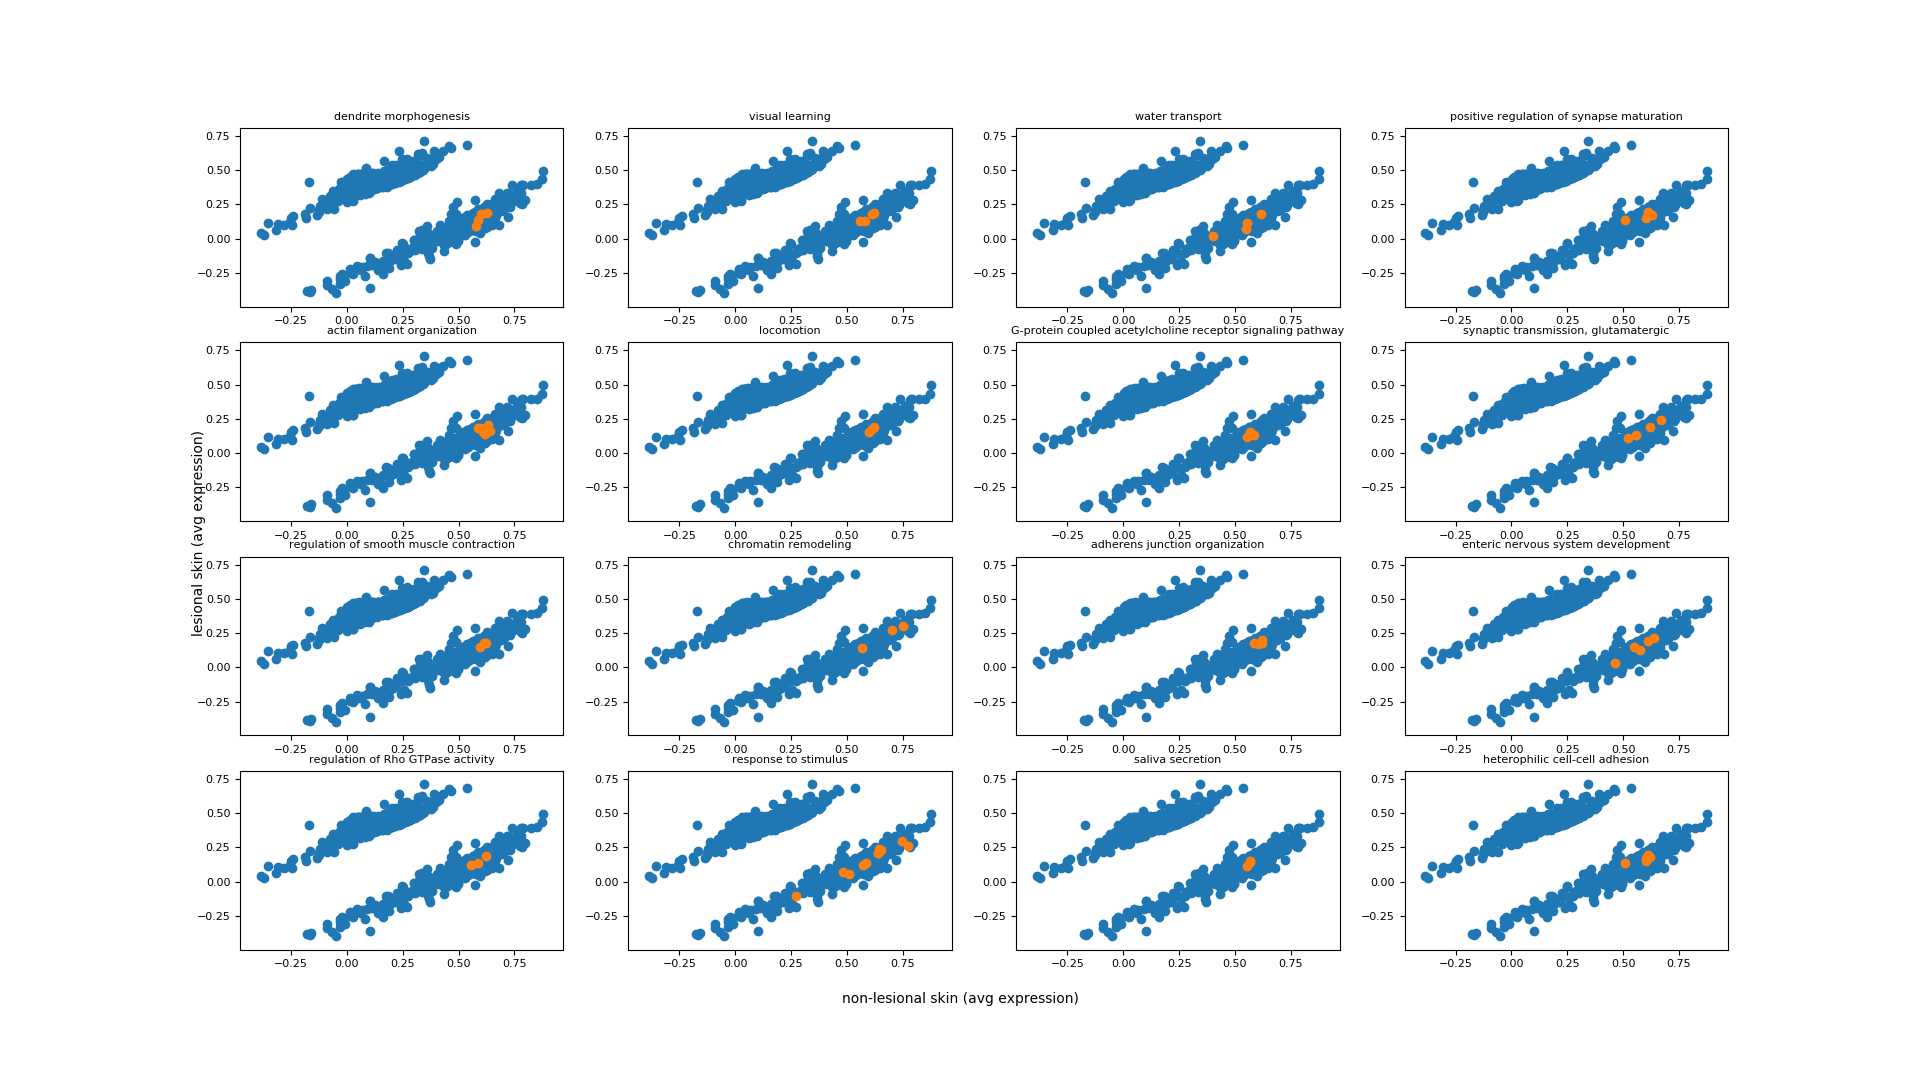
\includegraphics[width=1\textwidth]{Sign_Processes_Psoriasis_Scaled.png}
		\label{fig:ProcessesScaledByFeature}
		\caption{The 16 processes that showed the highest difference in gene expression between lesional and non-lesional data. The data is standardized by feature and orange points are genes that are related to the process, Blue dots are genes unrelated to the process}
	\end{figure}

	\begin{figure}[H]
		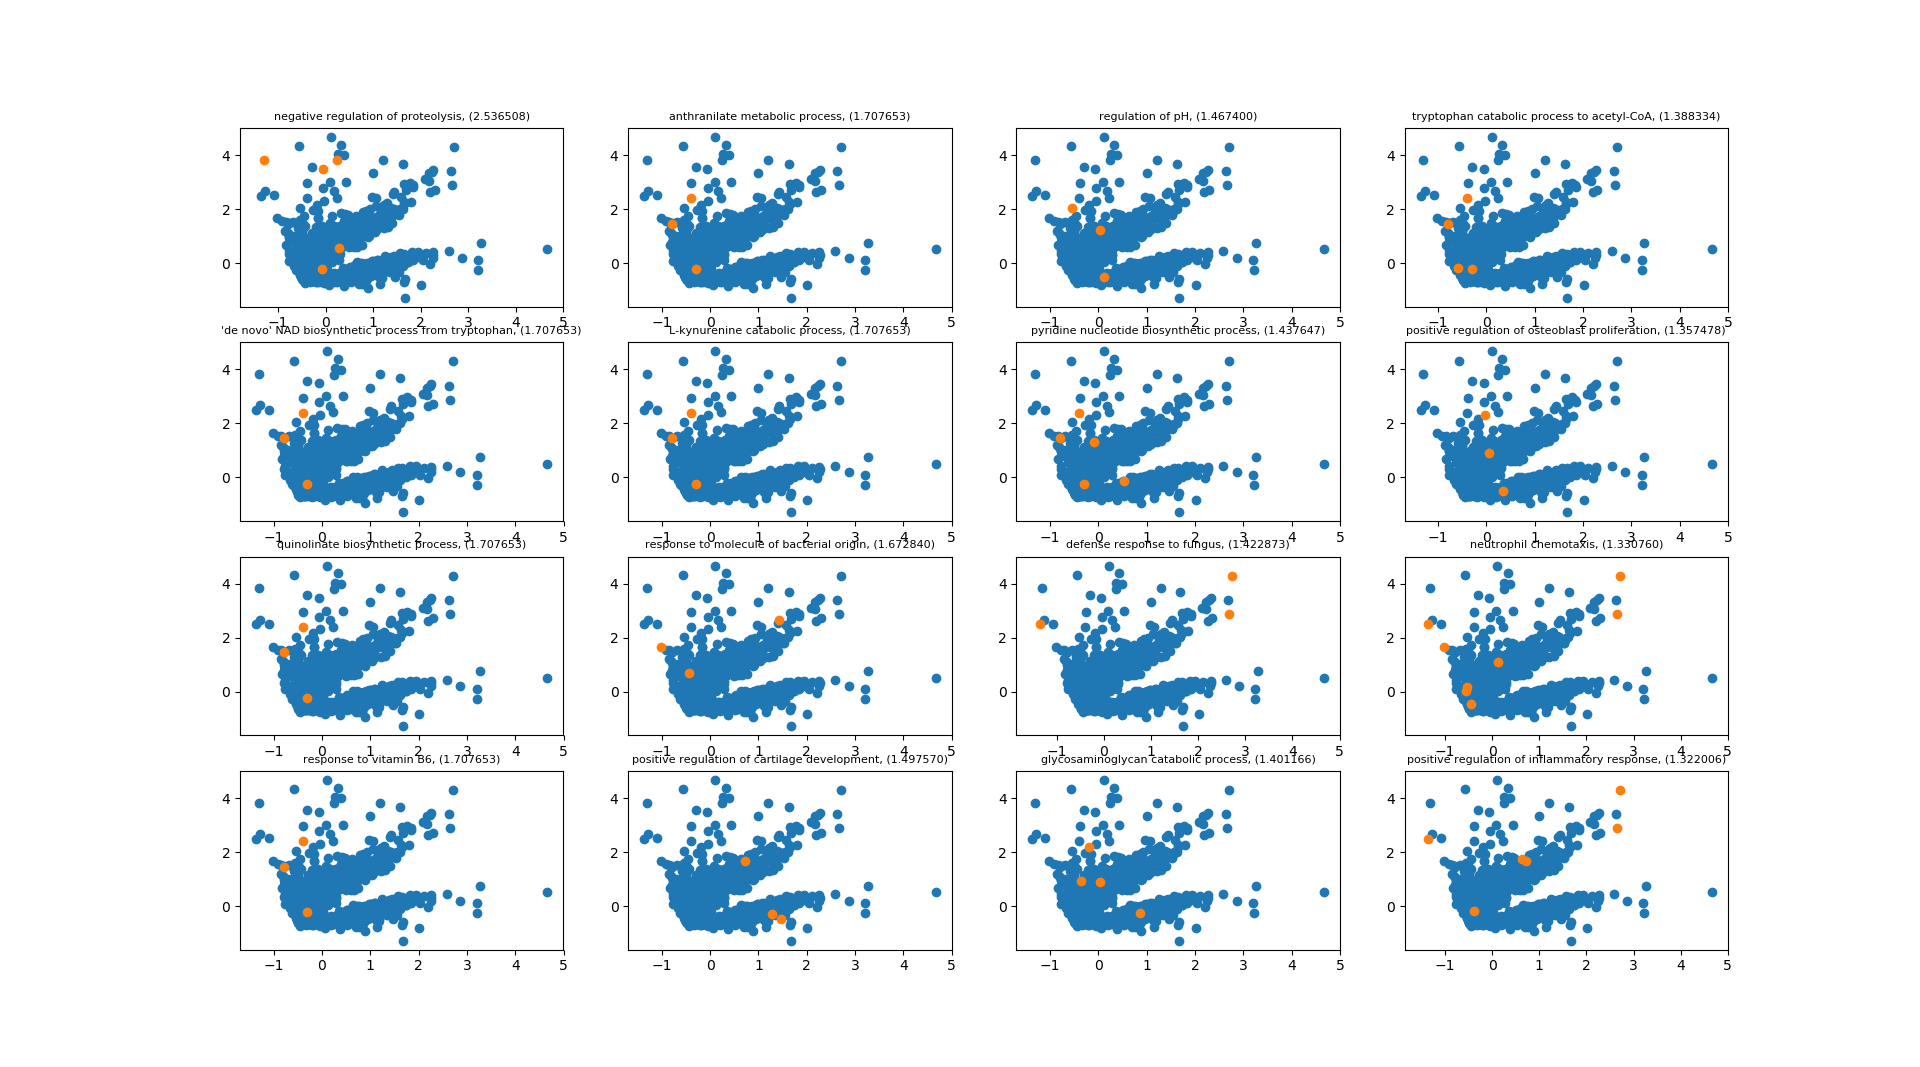
\includegraphics[width=1\textwidth]{Sign_Processes_Psoriasis.png}
		\label{fig:ProcessesScaledBySample1}
		\caption{The 16 processes that showed the highest difference in gene expression between lesional and non-lesional data. The data is standardized by sample and orange points are genes that are related to the process, Blue dots are genes unrelated to the process}
	\end{figure}
	
	\begin{figure}[H]
		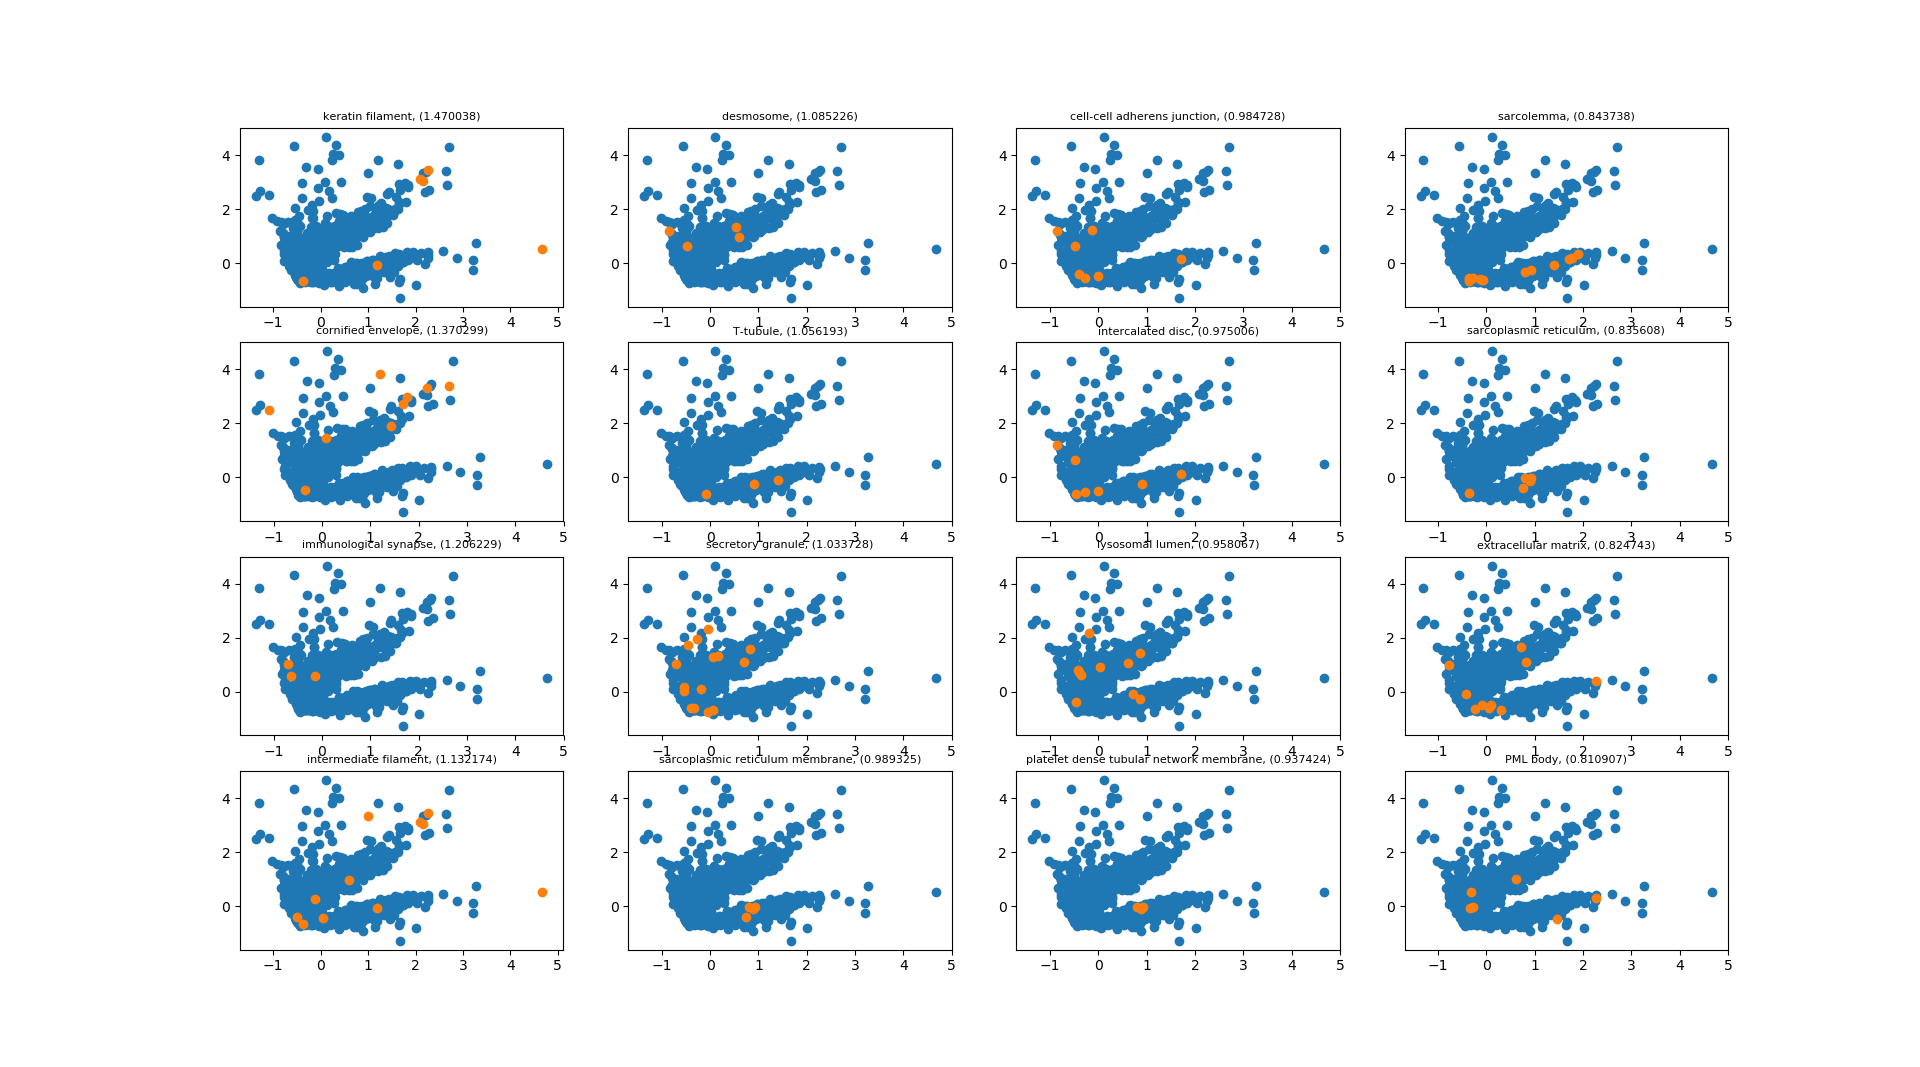
\includegraphics[width=1\textwidth]{Sign_Organelles_Psoriasis.png}
		\label{fig:CellularScaledBySample}
		\caption{The 16 cellular locations that showed the highest difference in gene expression between lesional and non-lesional data. The data is standardized by sample and orange points are genes that are related to the cellular location, Blue dots are genes unrelated to the cellular location}
	\end{figure}

	% Insert figures
	\begin{figure}[H]
		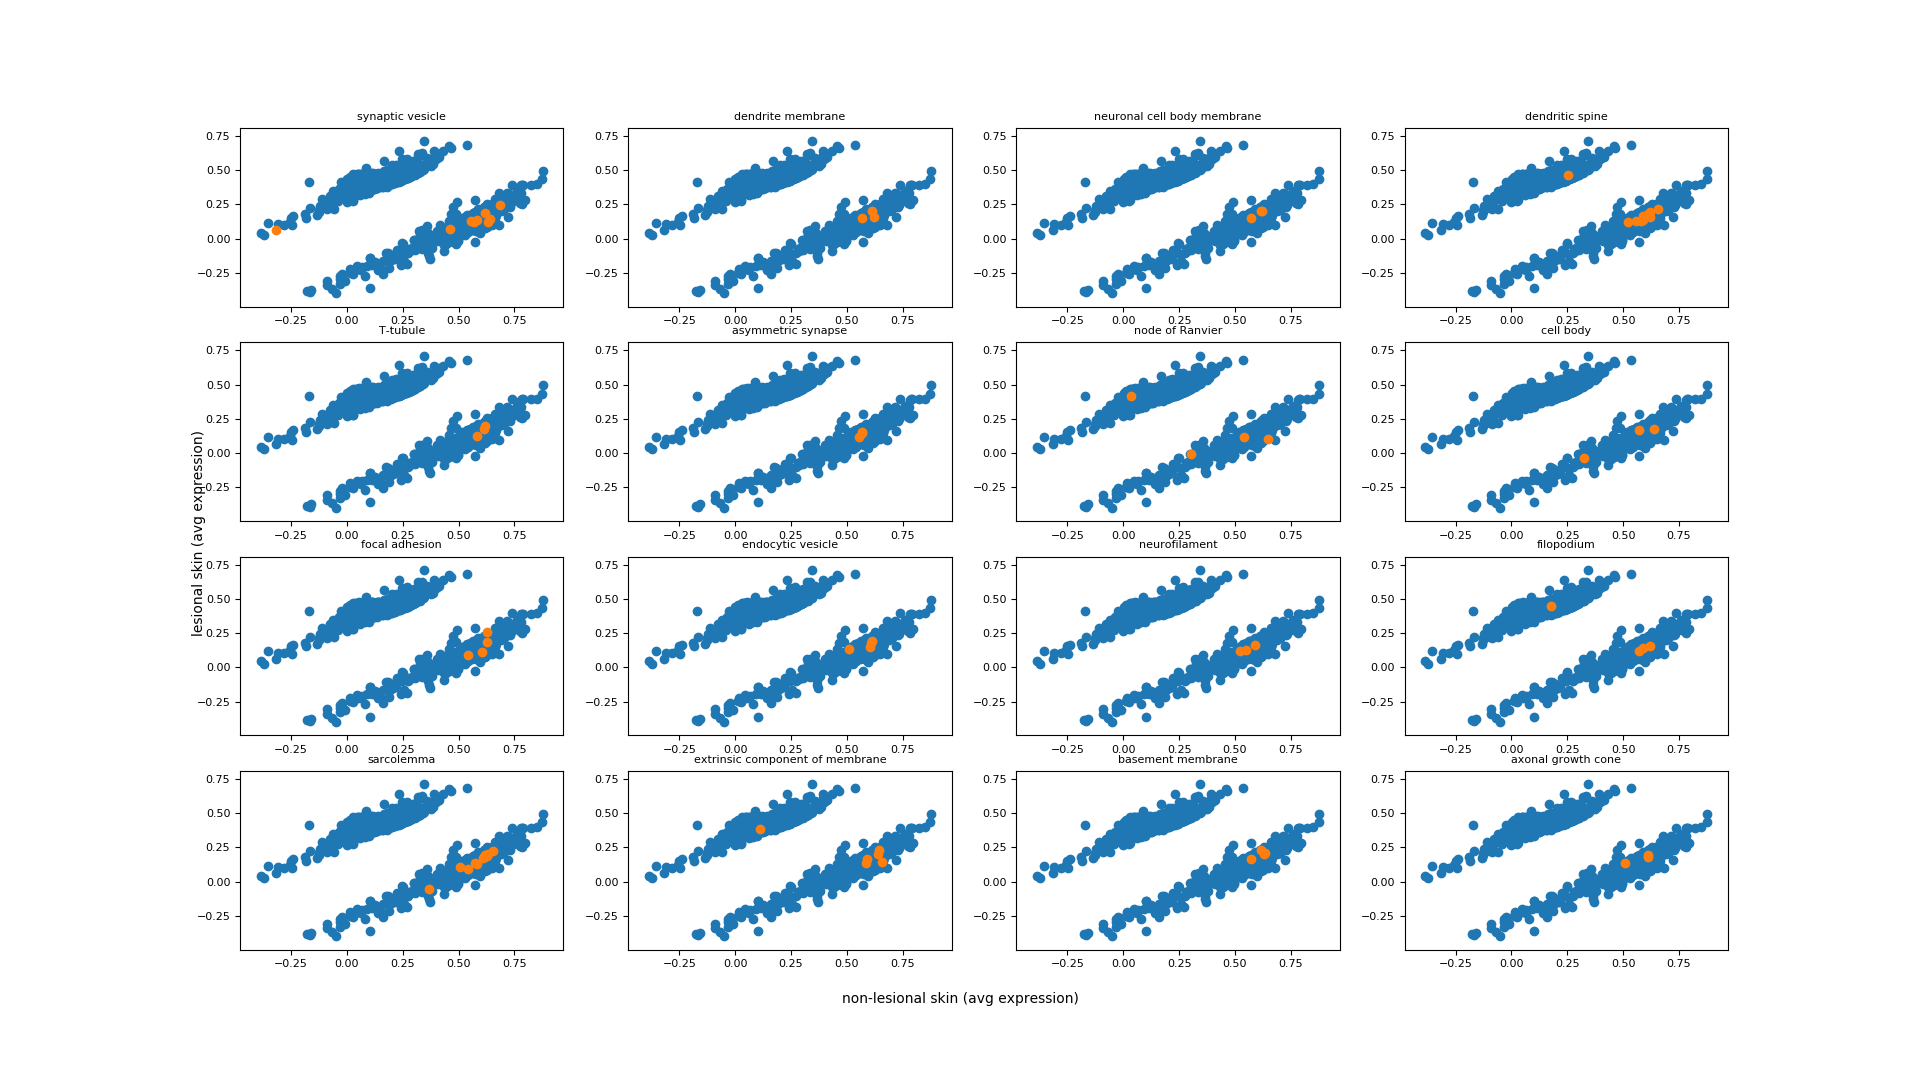
\includegraphics[width=1\textwidth]{Sign_Organelles_Psoriasis_Scaled.png}
		\label{fig:CellularScaledByFeature1}
		\caption{The 16 cellular locations that showed the highest difference in gene expression between lesional and non-lesional data. The data is standardized by feature and orange points are genes that are related to the cellular location, Blue dots are genes unrelated to the cellular location}
	\end{figure}

	\begin{figure}[H]
		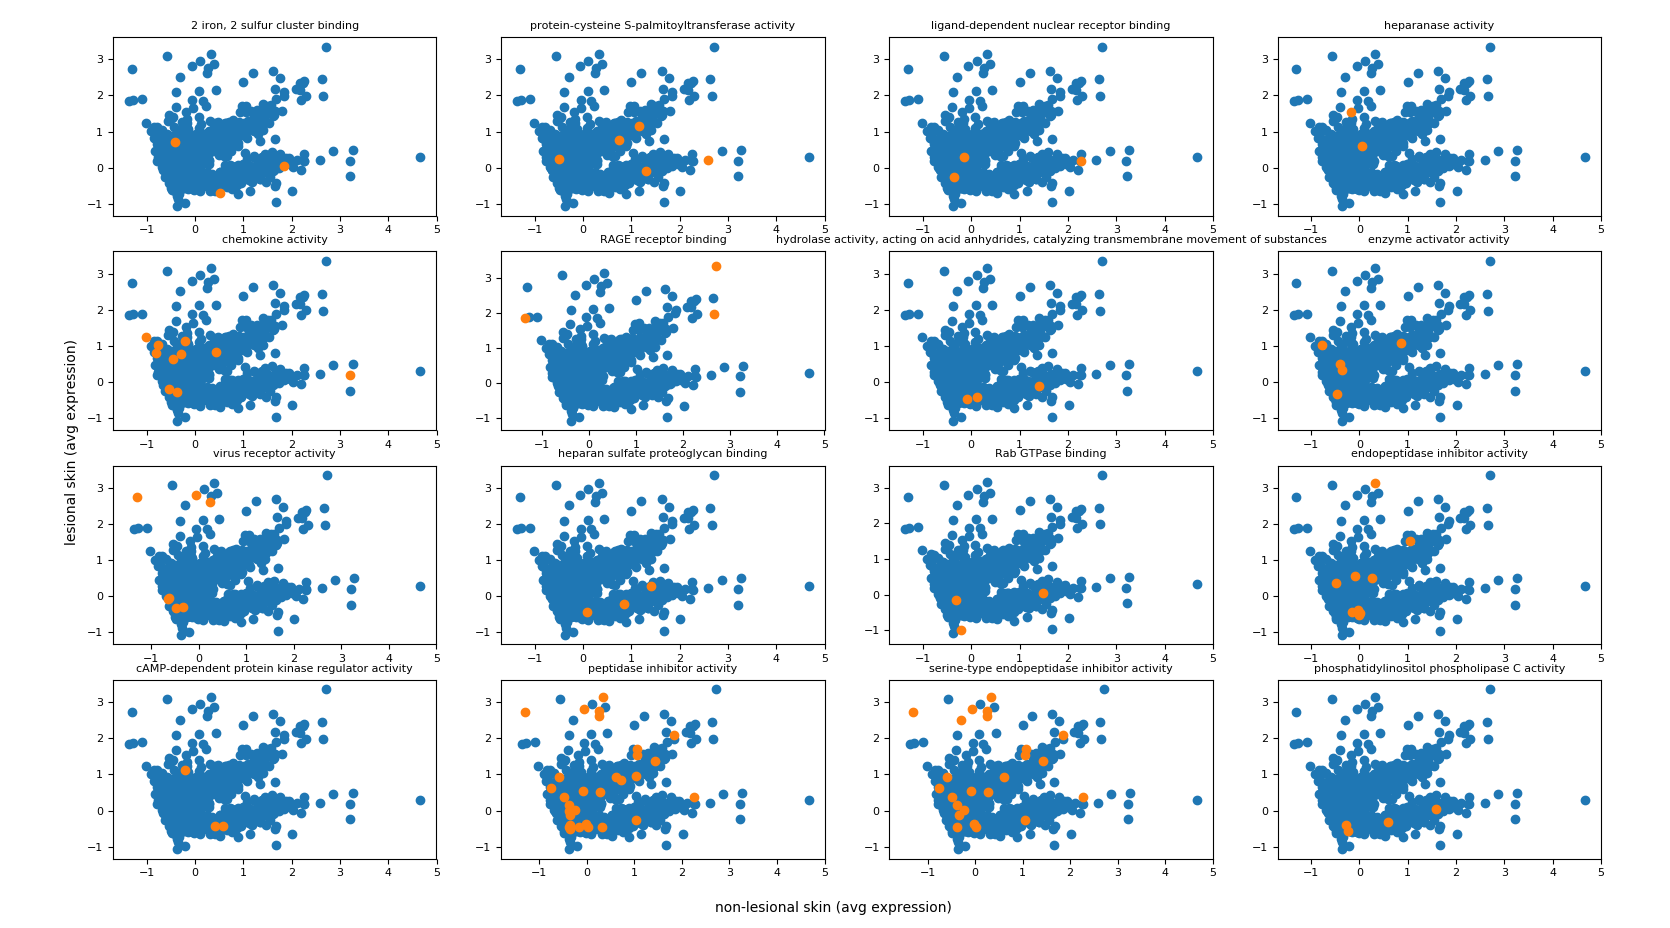
\includegraphics[width=1\textwidth]{Sign_Molecular_Psoriasis.png}
		\label{fig:MolecularScaledBySample}
		\caption{The 16 molecular relations that showed the highest difference in gene expression between lesional and non-lesional data. The data is standardized by sample and orange points are genes that are related to the molecular relation, Blue dots are genes unrelated to the molecular relation}
	\end{figure}
	
	% Insert figures
	\begin{figure}[H]
		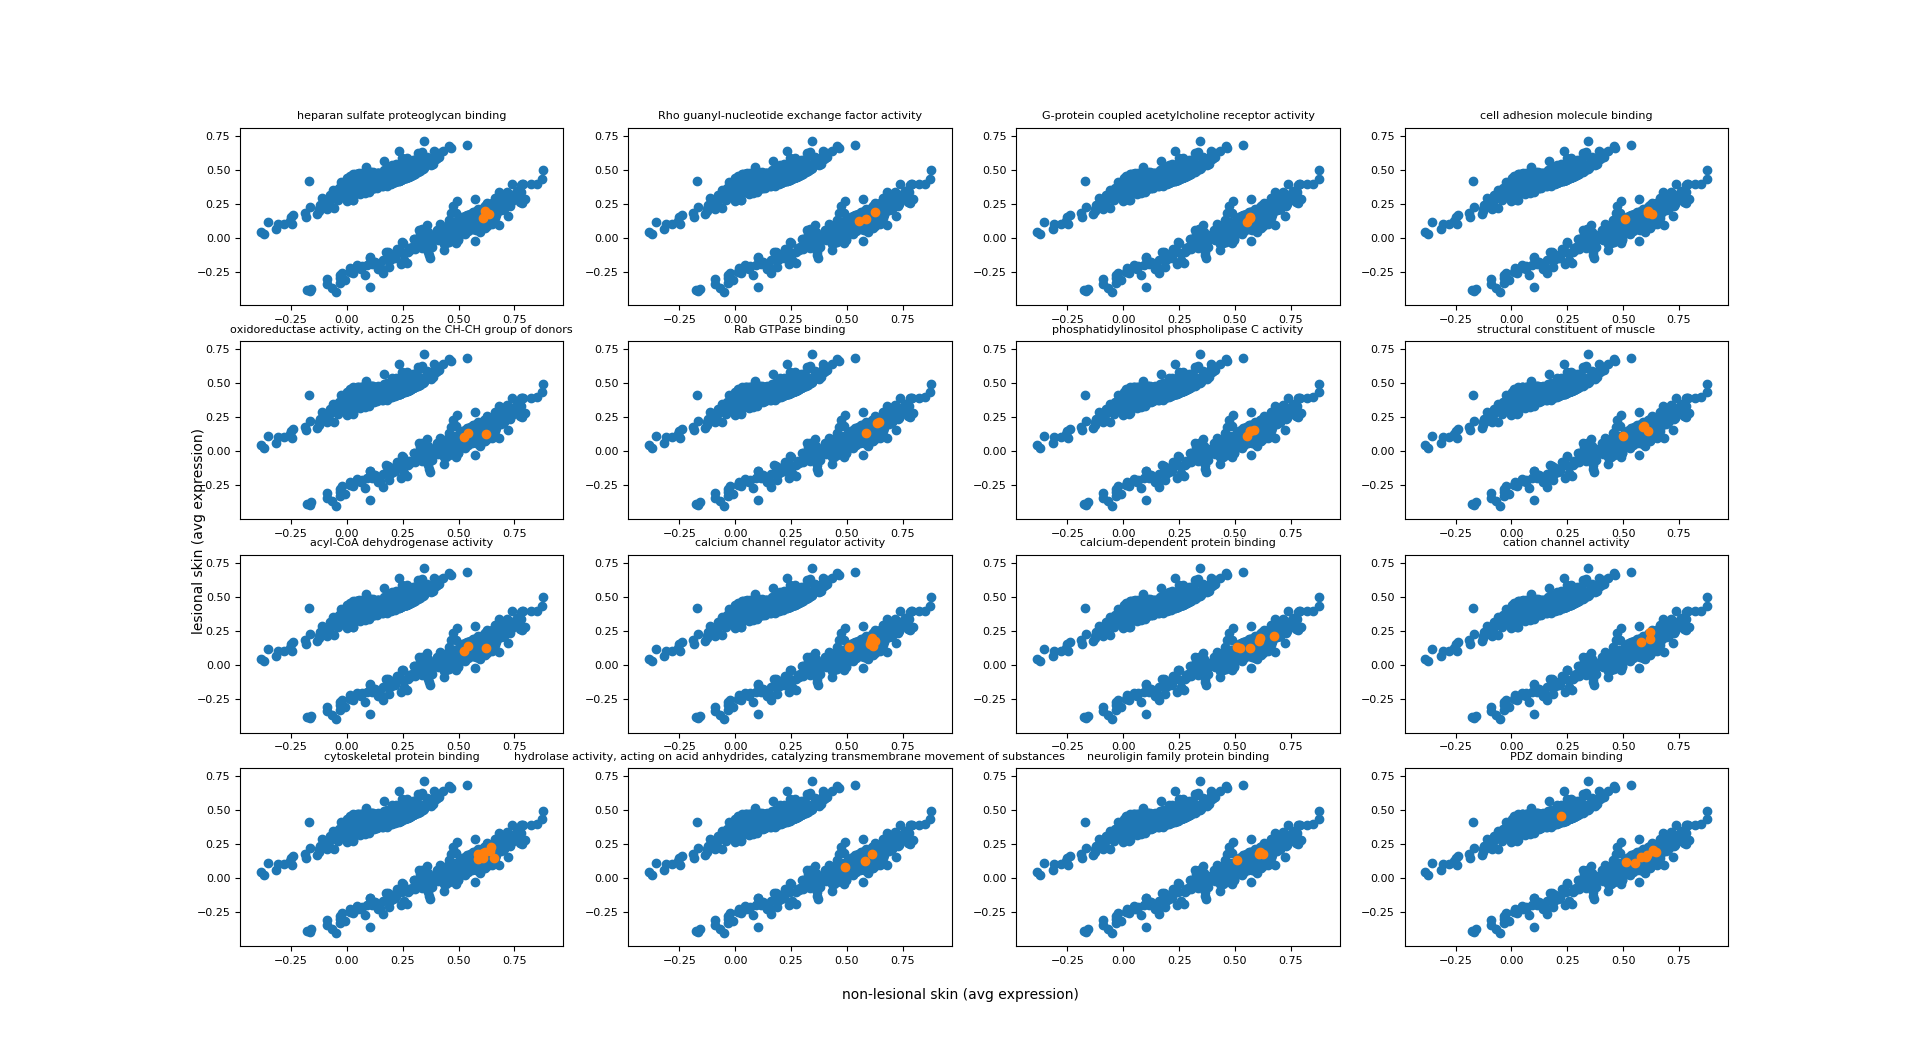
\includegraphics[width=1\textwidth]{Sign_Molecular_Psoriasis_Scaled.png}
		\label{fig:MolecularScaledByFeature1}
		\caption{The 16 molecular reactions that showed the highest difference in gene expression between lesional and non-lesional data. The data is standardized by feature and orange points are genes that are related to the molecular relation, Blue dots are genes unrelated to the molecular relation}
	\end{figure}


	
\end{document}
